% EMPIRICAL_MODEL_SUMMARY.tex
%
% photic's empirical model, MODEL lyzenga_log_linear: the fit, its depth error estimate, and the
% attenuation coefficients and physical depth from ATTENUATION, with their error estimate.
%
% Build: pdflatex EMPIRICAL_MODEL_SUMMARY.tex (twice, for the cross-references).

\documentclass[11pt]{article}
\usepackage{amsmath,amssymb,mathtools}
\usepackage[margin=2.5cm]{geometry}
\usepackage{booktabs}
\usepackage{graphicx}
\usepackage{xcolor}
\usepackage{hyperref}
\definecolor{dark-blue}{rgb}{0,0,0.45}
\hypersetup{colorlinks, linkcolor={dark-blue}, citecolor={blue}, urlcolor={blue}}

\numberwithin{equation}{section}

\newcommand{\bx}{\mathbf{x}}
\newcommand{\code}[1]{\texttt{#1}}
\newcommand{\Lsm}[1]{L_{\infty,#1}}

\title{The Empirical Model in \textit{photic}:\\
Lyzenga's Log-Linear Fit, Diffuse Attenuation and Depth Errors}
\author{Technical summary}
\date{20 October 2026}

\begin{document}
\maketitle

\begin{abstract}
\code{MODEL lyzenga\_log\_linear} fits Lyzenga's log-linear depth model to soundings, such as
ICESat-2 bathymetric photons. The model can be fitted to one image or to several scenes at once.
This note sets out how \textit{photic} makes three estimates.
\begin{enumerate}
\item The depth, and its 1$\sigma$ prediction error (\code{ERROR}), from a robust weighted
  least-squares fit.
\item The diffuse attenuation coefficient $K$ of every scene and band, as a smooth field over the
  scene (\code{ATTENUATION}, stage~1). It is estimated at the soundings, using the physical model
  that Lyzenga's regression linearises.
\item A physical depth at every cell, from how the attenuation differs between bands and scenes,
  with its own error estimate (stage~2).
\end{enumerate}
All of it is implemented in C, in \code{model/lyzenga.c}. The results quoted are from the
Arabian Gulf validation site between Dubai and Abu Dhabi: six Landsat~8 scenes, against
ICESat-2 ATL24 split by pass into calibration and test halves.

Lyzenga's fit across all scenes jointly scores 90.0\% hits on the test half. Its error estimate
holds 80\% of the errors within $\pm1\sigma$, but its tails are heavier than Gaussian. $K$ at
443--561\,nm is plausible and spatially coherent. $K$ at 655\,nm falls below pure water's
absorption, so it is not physical. The depth from the attenuation is a diagnostic, not a
product, and its error estimate is too small by a factor of about two to three.
\end{abstract}

\tableofcontents

%============================================================================================
\section{Notation and inputs}
\label{sec:inputs}

\paragraph{Grids.} The command takes $n$ band grids $L_m$, $m = 1,\dots,n$, all on one grid. They
can be remote-sensing reflectance from ACOLITE, or radiance. With \code{ATTENUATION ...\ SCENES}
$S$, the grids are scene-major: $S$ scenes of $n_b = n/S$ bands each, in the same band order.
Grid $m$ belongs to scene $s(m) = \lfloor m/n_b \rfloor$.

\paragraph{Window means.} Each band is averaged over a $(2r-1)\times(2r-1)$ window of valid cells
(\code{RADIUS} $r$), giving $\bar L_m(\bx)$. A cell is modelled only where every band is valid.
\code{LAND} and \code{SHALLOW} masks, if given, further restrict it.

\paragraph{Deep-water signal and noise.} For each band:
\begin{itemize}
\item $\Lsm{m}$ is either given (\code{LSM}) or the $p$-th percentile of the window means
  (\code{PERCENTILE}, default $p = 1$).
\item $\sigma_m$ is the robust spread of the darkest cells: $1.4826$ times the median absolute
  deviation of the window means at or below that percentile. It stands for the noise of a
  deep-water cell.
\end{itemize}
The signal above deep water is
\begin{equation}
  v_m(\bx) = \bar L_m(\bx) - \Lsm{m} .
\end{equation}
A band sees the bottom while $v_m \ge k\,\sigma_m$ (\code{DEEP} $k$, default 2). A cell where any
band fails this test is optically deep for the Lyzenga fit, and gets no depth.

\paragraph{Soundings and tides.} Soundings $z$ are depths below the datum, positive down. Each
sounding goes to its nearest cell; only soundings within \code{DEPTHS} $[z_{\min}, z_{\max}]$
are used. \code{TIDE} $h$ is the water level above the datum when the image was taken, so the
light saw a water column $Z = z + h$. With several scenes, scene $s$ has its own level $h_s$
(\code{TIDES}), and $Z_s = z + h_s$. Outputs are depths below the datum, negative down.

The soundings file must hold depths below the datum. If the tide is added both to the file and
through \code{TIDE}, it is counted twice; this happened in the Gulf composite runs and was
fixed on 20 October 2026.

%============================================================================================
\section{Lyzenga's regression}
\label{sec:lyzenga}

\subsection{The model and its fit}

With $X_m = \ln v_m$, the model (Lyzenga 1978, 1985; Lyzenga et al.\ 2006) is
\begin{equation}
  \hat Z = a_0 + \sum_{m=1}^{n} a_m X_m = \mathbf{a}^{\mathsf T}\mathbf{x},
  \qquad \mathbf{x} = (1, X_1, \dots, X_n)^{\mathsf T}.
  \label{eq:lyzenga}
\end{equation}
Setting \code{LSM 0} gives the plain $\ln L$, with no deep-water signal subtracted; Lyzenga et
al.\ (2006) always subtract one. Fitted to every scene's bands at once,
equation~\eqref{eq:lyzenga} is the \emph{joint} model. It includes every weighted sum of per-scene
fits as a special case. The scenes' tides are constants per scene, so they go into the
coefficients, and the target is depth below the datum (\code{TIDE 0}).

The rows are the $N$ soundings whose cells see the bottom in every band. The coefficients
minimise
\begin{equation}
  \sum_{i=1}^{N} w_i \bigl(Z_i - \mathbf{a}^{\mathsf T}\mathbf{x}_i\bigr)^2 ,
\end{equation}
solved by Householder QR of $W^{1/2}A$, which gives the triangular factor $R$ with
$R^{\mathsf T}R = A^{\mathsf T}WA$. The weights are $w_i = w_i^{0}\,\psi_i$:
\begin{itemize}
\item $w_i^{0}$ is 1, or $1/(\text{count in the sounding's depth bin})$ with \code{BALANCE}.
\item $\psi_i$ are Huber weights, from iteratively reweighted least squares:
  $\psi_i = \min\bigl(1,\; k_H s / |e_i|\bigr)$, where $e_i$ is the residual,
  $s = 1.4826\,\mathrm{median}|e_i|$, and $k_H = 1.345$ (\code{HUBER}). The iterations start
  from the least-squares solution.
\end{itemize}

\subsection{Rescaling against regression dilution (\code{POWER})}

Noise in the predictors shrinks the fitted depths towards the mean, so deep water reads too
shallow. \code{POWER} uses classical calibration to correct this:
\begin{enumerate}
\item At the soundings, the fit's depths are modelled as $\hat Z = c\,Z^{d}$, fitted robustly in
  logs: $\ln \hat Z = \ln c + d \ln Z$, with the same Huber IRLS.
\item The law is inverted: $Z' = (\hat Z/c)^{1/d}$.
\end{enumerate}
By default, the inverse is applied only beyond the crossover $\hat Z_\times = c^{1/(1-d)}$. That is
where the fit is compressed into too little depth, so shallow depths keep the fit's smaller
scatter. \code{POWER ALL} applies the inverse at every depth. At the Gulf, the joint fit gives
$\hat Z = 1.081\,Z^{0.959}$, with the crossover at 6.9\,m.

\subsection{The depth error estimate (\code{ERROR})}
\label{sec:lyz_error}

The \code{ERROR} grid is the 1$\sigma$ prediction error of a new depth at cell $\bx$. Write $W$
for the final weights, rescaled to average 1 ($\tilde w_i = N w_i / \sum_j w_j$). The residual
variance of a sounding of average weight is
\begin{equation}
  s^2 = \frac{1}{N - p}\sum_{i=1}^{N} \tilde w_i\, e_i^2 , \qquad p = n + 1 .
  \label{eq:s2}
\end{equation}
The coefficients' covariance follows from the QR factor:
\begin{equation}
  C = s^2 \bigl(A^{\mathsf T}\tilde W A\bigr)^{-1} = s^2\,\frac{\sum_j w_j}{N}\,(R^{\mathsf T}R)^{-1}.
\end{equation}
The prediction variance at a cell with predictors $\mathbf{x}$ is then
\begin{equation}
  \sigma_{\hat Z}^2(\bx) = s^2 + \mathbf{x}^{\mathsf T} C\, \mathbf{x} .
  \label{eq:pred_var}
\end{equation}
It has two parts: the scatter of one sounding about the model, and the uncertainty of the
coefficients, which grows as $\mathbf{x}$ moves away from the soundings' centre.

Through \code{POWER}, a small error in $\hat Z$ scales by $\mathrm{d}Z'/\mathrm{d}\hat Z =
Z'/(d\,\hat Z)$. So where the rescaling applies,
\begin{equation}
  \sigma_{Z'} = \sigma_{\hat Z}\, \frac{Z'}{d\,\hat Z} .
\end{equation}

\paragraph{What it represents.} Because Huber weighting is used, $s^2$ in~\eqref{eq:s2} is a robust
variance. Outlying soundings are down-weighted, so $s$ (0.70\,m at the Gulf) describes the core
of the residuals, not their tails (in-sample rms 1.86\,m). The estimate assumes
\begin{itemize}
\item residuals independent between soundings, with one variance at every depth and place;
\item the model's form is right.
\end{itemize}
It therefore cannot see:
\begin{itemize}
\item saturation where the bands stop seeing the bottom;
\item spatially correlated error, for example from a change of bottom type;
\item errors in the soundings themselves.
\end{itemize}

\paragraph{Calibration at the Gulf.} This is the joint model, four bands per scene, with
\code{POWER}, scored against ICESat-2 cells that the fit did not use (Table~\ref{tab:lyz_error}).
\begin{itemize}
\item \textbf{The core is conservative:} 80\% of the errors lie within $\pm1\sigma$, against 68\%
  for a Gaussian.
\item \textbf{The tails are heavy:} 93.6\% lie within $\pm2\sigma$, against 95\%. The rms of
  $e/\sigma$ is 1.6.
\item \textbf{$\sigma$ hardly varies:} it is 0.70--0.76\,m at every depth, because
  $\mathbf{x}^{\mathsf T}C\mathbf{x}$ is small next to $s^2$ for 6,017 soundings.
\item \textbf{It misses the saturation:} below about 16\,m, the 20--30\,m cells have no errors
  within $\pm1\sigma$.
\end{itemize}
So it is a fair guide to the typical error in the depths the model reaches. It is not a bound,
and it says nothing about saturation.

\begin{table}[h]
\centering
\caption{Calibration of Lyzenga's \code{ERROR} on the Gulf's test half (joint model, four bands,
\code{POWER}; 5,543 cells with a depth). Overall, 93.6\% of the errors lie within $\pm2\sigma$.}
\label{tab:lyz_error}
\begin{tabular}{lrrrr}
\toprule
Depth (m) & Cells & Within $\pm1\sigma$ & Median $\sigma$ (m) & RMSE (m) \\
\midrule
0--2   & 161   & 83\% & 0.70 & 2.38 \\
2--5   & 1,352 & 87\% & 0.70 & 1.32 \\
5--10  & 2,027 & 79\% & 0.74 & 0.78 \\
10--20 & 1,980 & 77\% & 0.75 & 0.97 \\
20--30 & 23    & 0\%  & 0.76 & 8.77 \\
\midrule
All    & 5,543 & 80\% & 0.74 & 1.21 \\
\bottomrule
\end{tabular}
\end{table}

\begin{figure}[h]
\centering
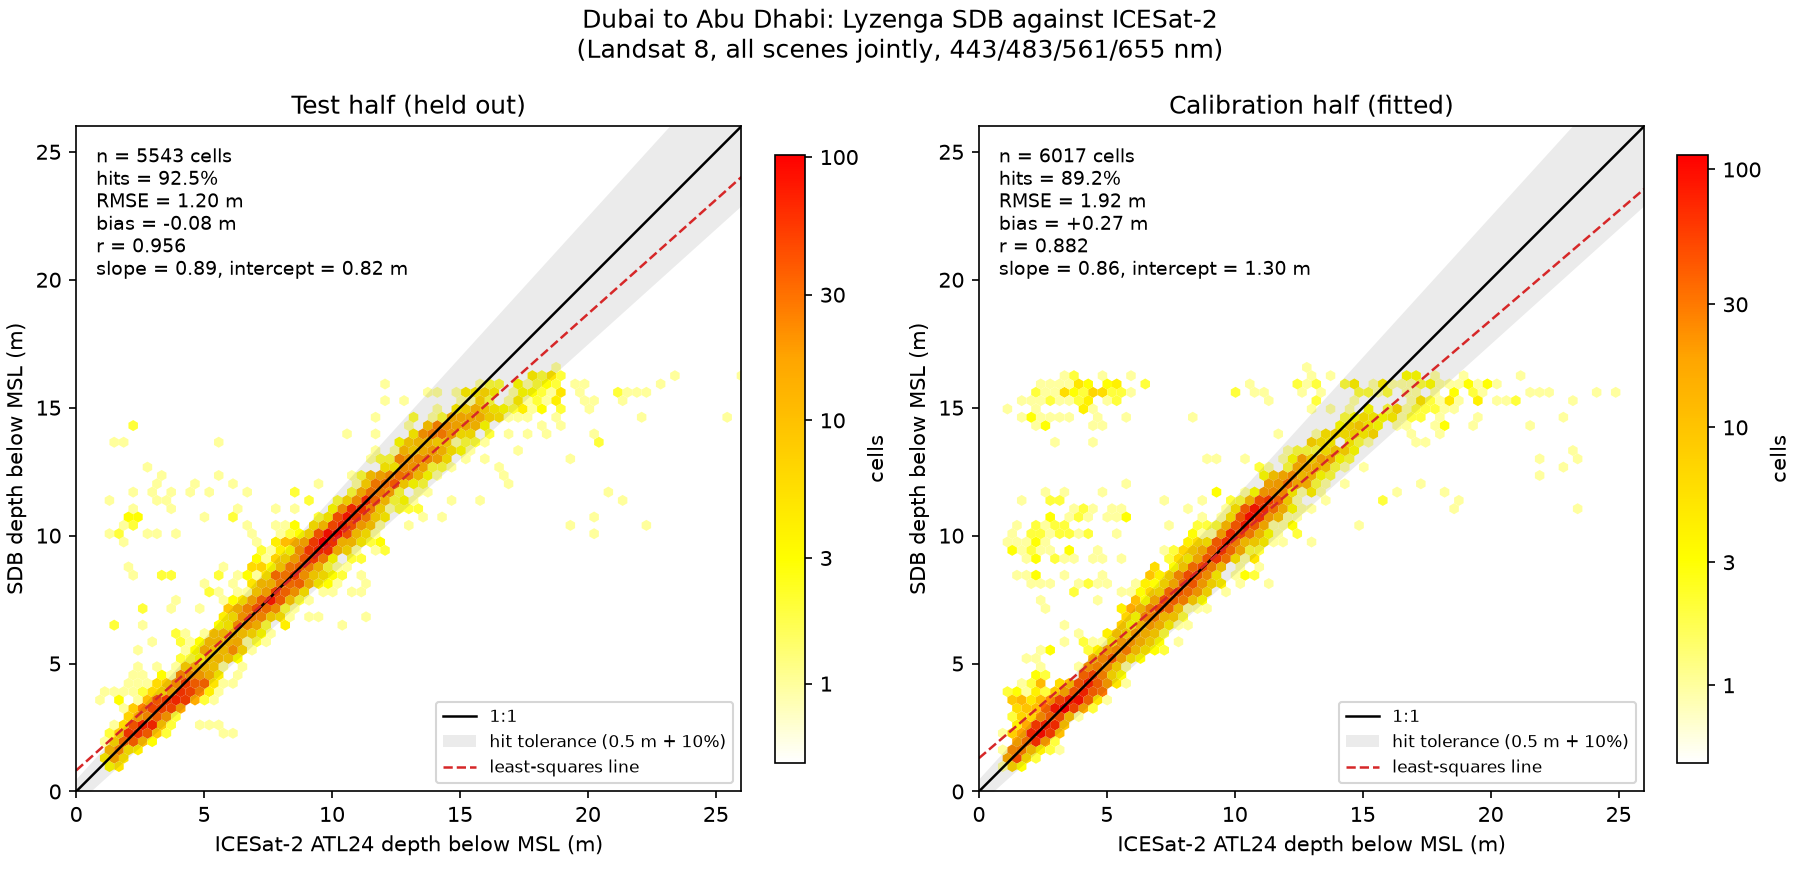
\includegraphics[width=\textwidth]{paper/empirical_figures/lyzenga_correlation.png}
\caption{The joint Lyzenga model against ICESat-2 at the Gulf. The test half is held out by
pass; the calibration half was fitted. Hits here count cells with a depth. Counting every
reference cell, the test-half score is 90.0\%.}
\label{fig:lyz}
\end{figure}

%============================================================================================
\section{The attenuation behind the regression}
\label{sec:physics}

Lyzenga's model is the linearisation of a two-flow model of the water-leaving signal over an
optically shallow bottom:
\begin{equation}
  L_m - \Lsm{m} \;\approx\; A(\bx)\, r_m\, \exp\!\bigl(-g_m(\bx)\, Z_s\bigr),
  \qquad
  g_m = K_m\, M_s ,
  \label{eq:twoflow}
\end{equation}
where
\begin{itemize}
\item $A(\bx)$ is the bottom's brightness, taken as spectrally flat in logs (Lyzenga's
  assumption);
\item $r_m$ is the band's bottom colour, together with the band's deep-water and surface
  constants;
\item $K_m$ is the effective diffuse attenuation of the band;
\item $M_s$ is the path length in water per metre of depth, down and back up.
\end{itemize}
$M_s$ comes from the sun and view zeniths in air (\code{SUNZENITH}, \code{VIEWZENITH}), refracted
into water with $n_w = 1.34$:
\begin{equation}
  M_s = \sec\theta_{w,\mathrm{sun}} + \sec\theta_{w,\mathrm{view}},
  \qquad \sin\theta_w = \sin\theta / n_w .
\end{equation}
With both zeniths at 0, $M_s = 2$. For the Gulf scenes (sun zenith 35--51\textdegree, near-nadir
view), $M_s$ is about 2.1--2.25.

If the down- and up-welling attenuations differ, $g_m = K_{d}\sec\theta_{w,\mathrm{sun}} +
K_{u}\sec\theta_{w,\mathrm{view}}$. The reported $K_m = g_m/M_s$ is then their path-weighted mean.

Taking logs of~\eqref{eq:twoflow} gives, for grid $m$ of scene $s$,
\begin{equation}
  X_m = \ln v_m = B(\bx) + c_m - g_m(\bx)\, Z_s ,
  \qquad B = \ln A, \; c_m = \ln r_m .
  \label{eq:logmodel}
\end{equation}
With $g_m$ and $c_m$ constant and $B$ constant, Lyzenga's regression~\eqref{eq:lyzenga} is this
equation solved for $Z$. In practice $g_m$ varies over a scene, and between scenes, with the
water. \code{ATTENUATION} estimates it explicitly, in two stages.

In stage~1, $\Lsm{m}$ is the \code{LSM} value where that is positive, and otherwise the
percentile. So \code{LSM 0} (the plain $\ln L$) still subtracts a deep-water signal for
the attenuation.

%============================================================================================
\section{Stage 1: the attenuation coefficients at the soundings}
\label{sec:stage1}

\subsection{A smooth field for each grid}

At the soundings the depth is known, so for each grid $m$ separately, equation~\eqref{eq:logmodel}
is fitted with $B$ left in the residuals:
\begin{equation}
  X_{m,i} = c_m - g_m(\bx_i)\, Z_{s,i} + \varepsilon_{m,i}.
  \label{eq:stage1}
\end{equation}
$g_m(\bx)$ is a bilinear interpolant of values $\theta_{m,q}$ on a regular grid of nodes, set
\code{NODES} degrees apart (default 0.05\textdegree; $12\times9$ nodes over the Gulf box):
\begin{equation}
  g_m(\bx) = \sum_{q=1}^{4} f_q(\bx)\, \theta_{m,q(\bx)} ,
\end{equation}
where $q(\bx)$ are the four nodes around the cell and $f_q$ their bilinear weights. The unknowns,
$c_m$ and the $Q$ node values $\theta_{m,\cdot}$, minimise
\begin{equation}
  \sum_{i} w_{m,i}\Bigl(X_{m,i} - c_m + Z_{s,i}\sum_q f_q(\bx_i)\theta_{m,q}\Bigr)^2
  \;+\; \lambda \sum_{(q,q')} \bigl(\theta_{m,q} - \theta_{m,q'}\bigr)^2 .
  \label{eq:stage1_obj}
\end{equation}
The second sum runs over neighbouring pairs of nodes, east--west and north--south. It is a
first-difference smoothing penalty, which makes the field smooth and fills nodes without
soundings. Its weight is scaled to an average node's data:
\begin{equation}
  \lambda = w_s \,\frac{\sum_i w^{0}_{m,i} Z_{s,i}^2}{Q},
\end{equation}
where $w_s$ is \code{SMOOTHING} (default 1; 0 requires soundings near every node). The normal
equations, of size $Q + 1$, are symmetric positive definite and are solved by Cholesky
factorisation. The residuals are robustified by the same Huber IRLS as in
Section~\ref{sec:lyzenga}, with scale $1.4826\,\mathrm{median}|\varepsilon|$.

\subsection{Weights from the noise}

The noise $\sigma_m$ on $v_m$ gives $\ln v_m$ a variance of about $\sigma_m^2/v_m^2$ (delta
method). This grows without limit as the signal sinks towards the deep-water level. A floor
$\epsilon = 0.05$ stands for the model's own error in $\ln v$. The weights are
\begin{equation}
  w^{0}_{m,i} = \Bigl(\frac{\sigma_m^2}{v_{m,i}^2} + \epsilon^2\Bigr)^{-1},
  \label{eq:weights}
\end{equation}
so a band counts fully while it sees the bottom clearly, and fades out as it loses it. The
Huber factors multiply $w^{0}$.

\subsection{Selecting soundings by the fitted signal}

A sounding enters grid $m$'s fit only while its signal is above the noise, $v \ge k\sigma_m$.
Selecting, and weighting, by the \emph{observed} signal truncates the data on the dependent
variable. At depth, only the cells that happen to be bright pass the test, which flattens the
slope and makes $K$ too small. The effect is largest in the red, which loses the bottom within a
few metres.

So after the first pass, each candidate sounding is reselected and reweighted by the
\emph{fitted} signal instead:
\begin{equation}
  \hat v_{m,i} = \exp\bigl(c_m - g_m(\bx_i)\, Z_{s,i}\bigr),
  \qquad \text{active if } \hat v_{m,i} \ge k\sigma_m,
\end{equation}
with $\hat v$ in place of $v$ in~\eqref{eq:weights}. The fit is repeated until the selection
stops changing, for at most 10 passes. This raised $K(655)$ at the Gulf by 20--40\%. A grid needs
at least 10 active soundings.

\subsection{Outputs}

\begin{itemize}
\item $K_m(\bx) = g_m(\bx)/M_{s(m)}$ at every valid cell, as grid \code{/prefix/\_/grid/}.
\item \code{attenuation.csv}: $K$ of every grid at every node, with the node's support (the sum
  of the bilinear weights of the soundings near it).
\item The printout gives, for each grid: $c_m$, the median $K$ over nodes with support of at
  least 1, its range, the robust scatter of~\eqref{eq:stage1}, and the number of passes.
\end{itemize}

\paragraph{Caveat.} $B$ is left in the residuals. $K$ is therefore unbiased only where the bottom's
brightness does not change systematically with depth across the soundings. If seagrass is
deeper than sand, the slope also contains the brightness change.

%============================================================================================
\section{Stage 2: a depth from the attenuation}
\label{sec:stage2}

\subsection{A straight line at every cell}

With $c_m$ and $g_m(\bx)$ fixed from stage~1, equation~\eqref{eq:logmodel} at a cell, over all its
grids, is a straight line in $g_m$:
\begin{equation}
  y_m \equiv X_m - c_m + g_m(\bx)\, h_{s(m)} = B(\bx) - g_m(\bx)\, H(\bx) ,
  \label{eq:stage2}
\end{equation}
where $H$ is the depth below the datum. The intercept $B$ is the bottom's brightness and the
slope is $-H$. The depth comes from how $g$ differs between bands and scenes, which is what makes
it independent of $B$.

The weighted least-squares line through the grids that see the bottom gives
\begin{equation}
  \hat H = -\frac{S_{gy}}{S_{gg}}, \qquad \hat B = \bar y + \hat H \bar g ,
\end{equation}
with
\begin{equation}
  \bar g = \frac{\sum w_m g_m}{\sum w_m}, \quad
  \bar y = \frac{\sum w_m y_m}{\sum w_m}, \quad
  S_{gg} = \sum_m w_m (g_m - \bar g)^2, \quad
  S_{gy} = \sum_m w_m (g_m - \bar g)(y_m - \bar y).
\end{equation}
The weights are~\eqref{eq:weights} with the cell's signal. As in stage~1, the first pass selects
and weights by the observed signal; later passes use the fitted signal,
\begin{equation}
  \hat v_m = \exp\bigl(\hat B + c_m - g_m(\hat H + h_{s(m)})\bigr) = v_m \exp\bigl(\hat B - g_m \hat H - y_m\bigr),
\end{equation}
until the selection settles (at most 10 passes). A cell needs at least 3 grids above
$k\sigma_m$.

The outputs are three grids:
\begin{itemize}
\item \code{/prefix/\_depth}, the depth $-\hat H$ (negative down);
\item \code{/prefix/\_depth\_sigma}, its error $\sigma_H$;
\item \code{/prefix/\_bottom}, the bottom brightness $\hat B$.
\end{itemize}

\subsection{The depth error estimate}
\label{sec:att_error}

$\sigma_H$ is the classical standard error of the slope of a weighted straight line, with the
residual scale estimated from the cell's own scatter about the line:
\begin{equation}
  \sigma_H = \sqrt{\frac{\mathrm{RSS}}{(n_u - 2)\,S_{gg}}}, \qquad
  \mathrm{RSS} = \sum_m w_m \bigl(y_m - \hat B + g_m \hat H\bigr)^2 ,
  \label{eq:sigmaH}
\end{equation}
where $n_u$ is the number of grids used.

The leverage is $S_{gg}$, the weighted spread of the two-way attenuation among the cell's grids.
It is small. Between 443 and 561\,nm, $K$ differs by only 0.01--0.03\,m$^{-1}$, so $g$ spans
about 0.02--0.07\,m$^{-1}$, and the scenes' different sun angles add little. A bottom colour that
departs from spectral flatness by $\delta$ in $\ln$ therefore moves the depth by about
$\delta/\Delta g$. For $\delta = 0.1$ that is 1.5--5\,m, comparable to the depths being estimated.

Equation~\eqref{eq:sigmaH} treats the $n_u$ residuals as independent, with a common scale. It
omits three things.
\begin{enumerate}
\item \textbf{Stage~1's uncertainty.} $c_m$ and $g_m(\bx)$ are taken as exact. Their errors are
  shared by every cell near the same nodes, so they are systematic, not random, and they do not
  average down.
\item \textbf{The bottom's colour.} A non-flat bottom spectrum gives each band its own offset in
  $y_m$. The same offset recurs in every scene, so the residuals are correlated across scenes,
  and with only a few distinct bands it can be fitted into the slope rather than showing up as
  scatter.
\item \textbf{Few effective degrees of freedom.} The 18--24 grids are only 3--4 distinct bands
  seen 6 times under similar water. $n_u - 2$ overstates the information.
\end{enumerate}
All three make $\sigma_H$ too small. Out of fold at the Gulf, only 25\% (four bands) and 37\%
(443, 483 and 561\,nm) of the errors lie within $\pm\sigma_H$, against 68\% for a calibrated
estimate.

Two corrections are possible:
\begin{itemize}
\item propagate stage~1's covariance (the Cholesky factor is at hand) into~\eqref{eq:sigmaH};
\item inflate $\sigma_H$ by a factor calibrated out of fold.
\end{itemize}
Neither is built.

%============================================================================================
\section{Results at the Gulf}
\label{sec:results}

\subsection{The attenuation coefficients}

Over the box, $K$ is 0.05--0.09\,m$^{-1}$ at 443\,nm, 0.07--0.10 at 483 and 0.065--0.105 at 561
(medians over the scenes), and it varies 1.5--2$\times$ across the box
(Figure~\ref{fig:kmaps}). The three bands are fitted independently, yet they map the same
pattern: low in the south-west, rising towards Jebel Ali and Dubai. The scenes differ:
2019-03-13 is the clearest, 2018-10-04 the least clear. One set of Lyzenga coefficients cannot
represent this variation. These maps are the per-site attenuation targets that the learned
model's physics decoder needs (\code{validation/FUTURE\_EXPERIMENTS.md}, H4(c)).

Pure water's absorption $a_w$ (Pope and Fry 1997) is a lower bound on $K$ (Figure~\ref{fig:kspec}).
\begin{itemize}
\item \textbf{443 and 483\,nm:} $K$ is 4--15 times $a_w$, as expected where dissolved and
  particulate matter dominate.
\item \textbf{561\,nm:} $K$ is barely above $a_w$ (0.065--0.105 against 0.062\,m$^{-1}$). 6\% of
  the node values fall below it, most of them in the clearest scene.
\item \textbf{655\,nm:} every value is below $a_w$ (0.08--0.19 against about 0.37\,m$^{-1}$), so
  none is physical.
\end{itemize}
The red loses the bottom within a few metres. Its deep-water signal varies (turbidity, adjacency,
the atmospheric residual) by far more than the darkest cells' spread $\sigma_m$, which sets the
threshold. So nearly every sounding stays active, and the slope is flattened. The flattening
already reaches the green on clear scenes.

Two remedies are possible, and neither is built:
\begin{itemize}
\item fit the deep-water level per grid, or as a field;
\item bound $K$ below by $a_w$.
\end{itemize}
A pure-water bound would bind at 561\,nm as well as at 655.

\begin{figure}[p]
\centering
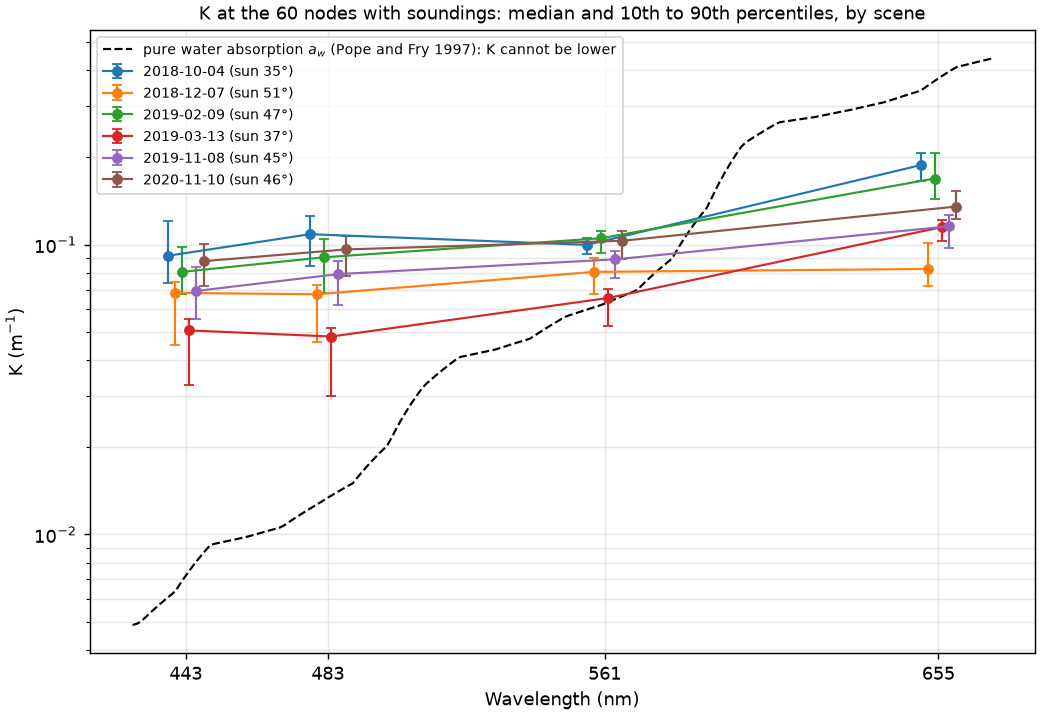
\includegraphics[width=0.8\textwidth]{paper/empirical_figures/k_spectra.png}
\caption{$K$ of each scene against wavelength at the 60 nodes with soundings (median, with the
10th to 90th percentiles), and pure water's absorption $a_w$. $K$ cannot physically fall below
$a_w$.}
\label{fig:kspec}
\end{figure}

\begin{figure}[p]
\centering
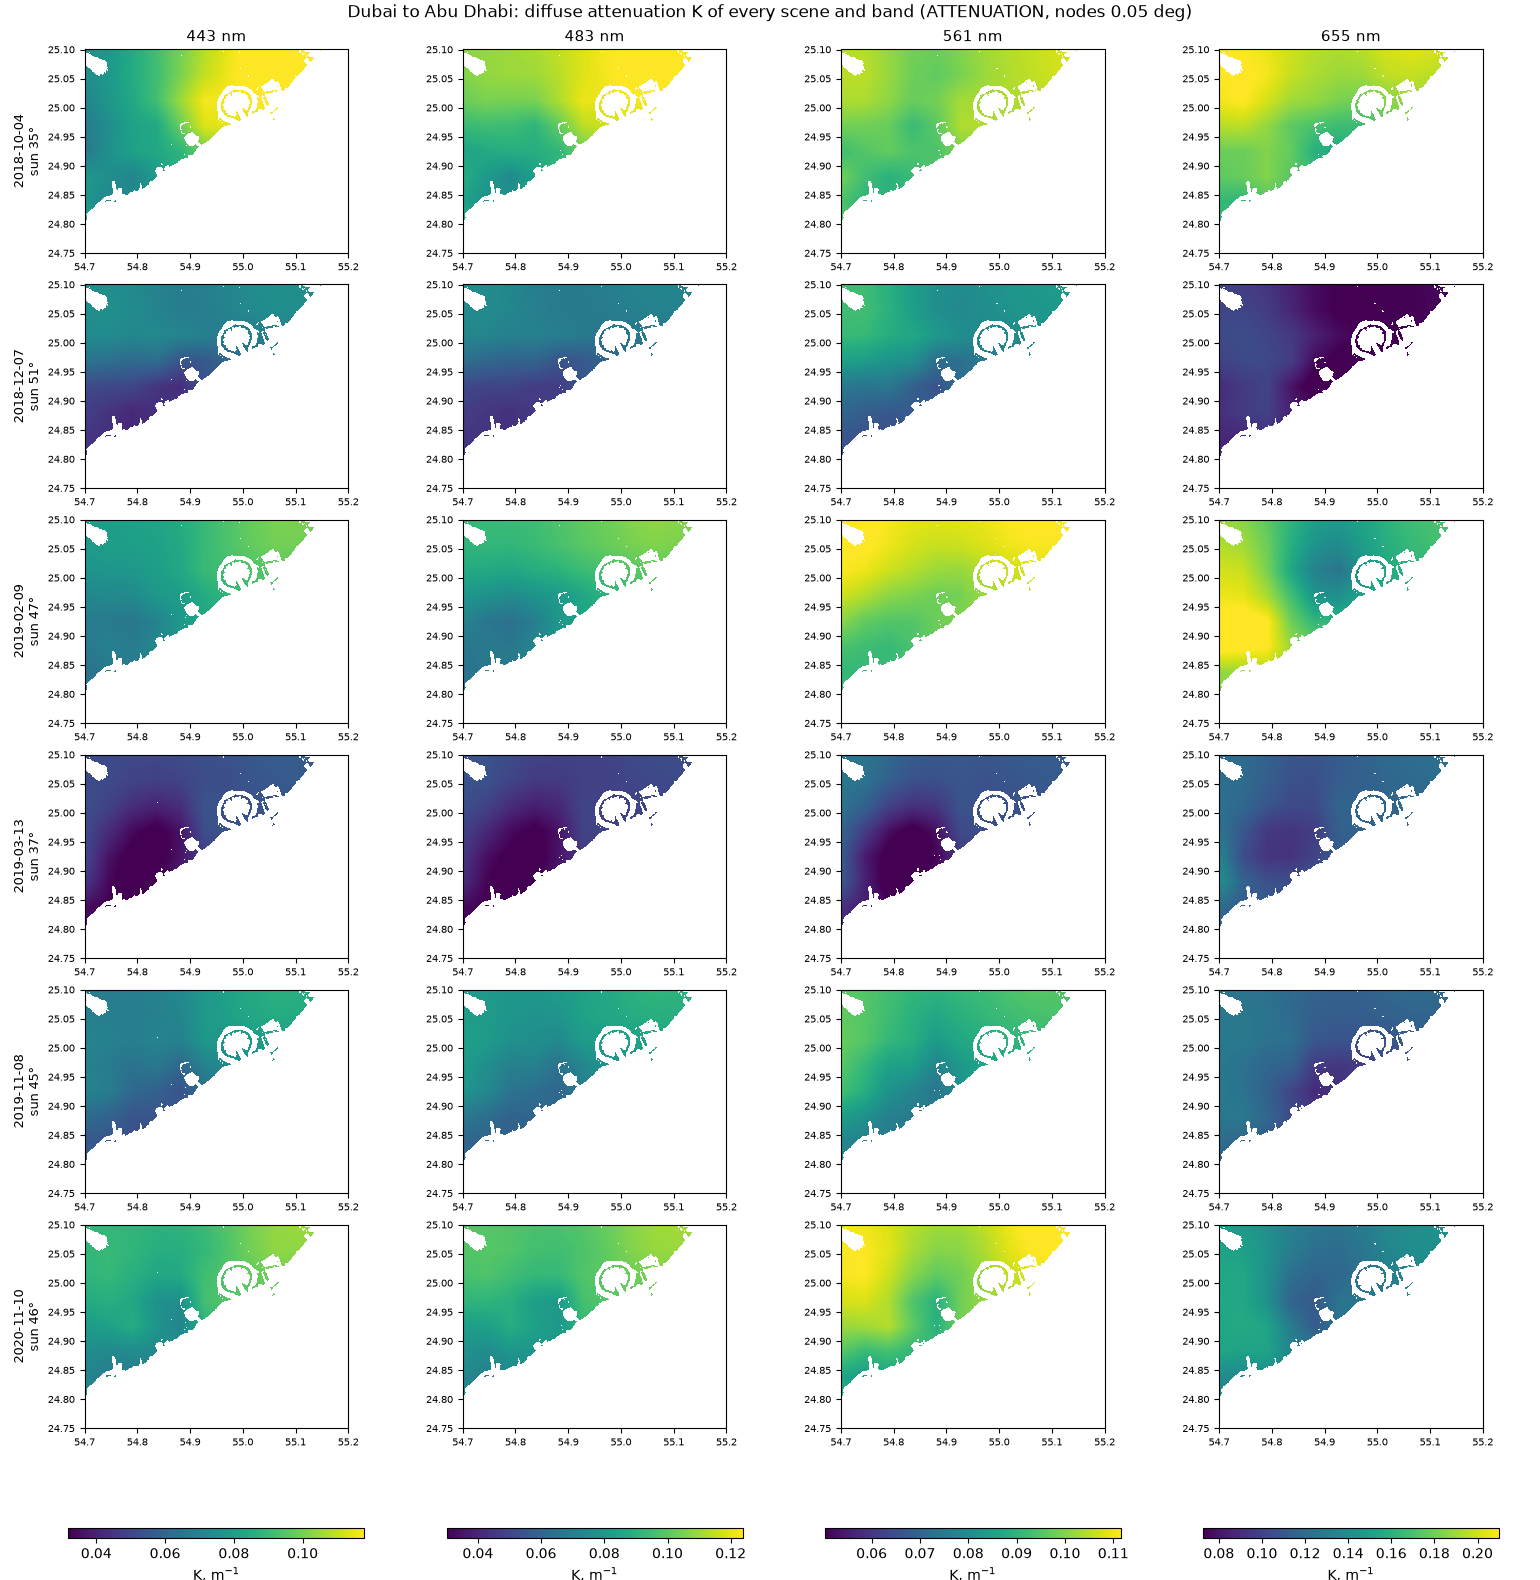
\includegraphics[width=\textwidth]{paper/empirical_figures/k_maps.png}
\caption{$K$ of every scene (rows, with the date and sun zenith) and band (columns), on one colour
scale per band. Nodes are 0.05\textdegree\ apart.}
\label{fig:kmaps}
\end{figure}

\subsection{The depth from the attenuation}

Table~\ref{tab:att} scores the depth from the attenuation against Lyzenga's depth, out of fold.
The folds are the four ICESat-2 pass groups that chose Lyzenga's settings, within the calibration
half only. The harness reproduces Lyzenga's cross-validation score (83.9\%).

\begin{table}[h]
\centering
\caption{Out of fold on the Gulf's calibration half (5,833 cells). A hit is an error within
$0.5\,\mathrm{m} + 10\%$ of the depth.}
\label{tab:att}
\begin{tabular}{lrrrrrrr}
\toprule
 & Hits & RMSE (m) & Bias (m) & 0--2 & 2--5 & 5--10 & 10--20 \\
\midrule
Lyzenga, joint, four bands     & 83.9\% & 2.09 & $+0.26$ & 58\% & 79\% & 90\% & 90\% \\
Attenuation depth, four bands  & 57.3\% & 3.14 & $-0.58$ & 5\%  & 56\% & 79\% & 47\% \\
Attenuation depth, 443/483/561 & 61.4\% & 2.84 & $+0.12$ & 34\% & 54\% & 69\% & 69\% \\
\bottomrule
\end{tabular}
\end{table}

The depth from the attenuation is not competitive with Lyzenga's. With so little spread in $g$,
a change of bottom type (seagrass against sand) shifts the band ratios enough to move the depth
by metres. Lyzenga's regression absorbs the site's bottom--depth relationships into its
coefficients; equation~\eqref{eq:stage2} cannot. Dropping the red removes the unphysical $K$ and
helps the shallowest water most (0--2\,m: 5 $\to$ 34\%). Its error estimate is too small
(Section~\ref{sec:att_error}).

So \code{ATTENUATION} is kept, off unless asked, with no effect on Lyzenga's fit. $K$ at
443--561\,nm is the usable product. The attenuation depth is a diagnostic.

%============================================================================================
\section{Usage}
\label{sec:usage}

\begin{verbatim}
MODEL lyzenga_log_linear GRIDS g1 ... gn BATHYMETRY H [options, any order]
  LSM l1 ... ln | PERCENTILE p    DEEP k    RADIUS r    DEPTHS zmin zmax
  TIDE h    HUBER k    BALANCE bin    POWER [ALL]    ERROR H_error
  ATTENUATION K SCENES S [TIDES h1 ... hS] [SUNZENITH t1 ... tS]
                         [VIEWZENITH t1 ... tS] [NODES deg] [SMOOTHING w]
\end{verbatim}

\code{SCENES} must come before the per-scene lists, and the grids are scene-major. The outputs are:
\begin{itemize}
\item \code{H} and \code{H\_error};
\item with \code{ATTENUATION}, \code{K\_/grid/} for every grid, and \code{K\_depth},
  \code{K\_depth\_sigma} and \code{K\_bottom};
\item the files \code{model.bam} (the fitted model as applied), \code{output.csv} (every sounding,
  its model depth and whether it was used) and \code{attenuation.csv}.
\end{itemize}

At the Gulf, \code{validation/gulf\_lyzenga.py} runs it. That script prepares the inputs, chooses
the settings by cross-validation, scores the results and draws the figures; the modelling is all
in \textit{photic}. \code{make test} checks the fit and the attenuation on synthetic data that
follow the models exactly:
\begin{itemize}
\item \code{tests/lyz\_*}: the coefficients and every sounding's depth;
\item \code{tests/att\_*}: $K$ at every node, to $3\times10^{-6}$, and the depth at every cell,
  within 5\,mm (the float precision of the band grids).
\end{itemize}

\section*{References}

\begin{itemize}
\item Lyzenga, D.\,R. (1978). Passive remote sensing techniques for mapping water depth and
  bottom features. \textit{Applied Optics} 17(3), 379--383.
\item Lyzenga, D.\,R. (1985). Shallow-water bathymetry using combined lidar and passive
  multispectral scanner data. \textit{International Journal of Remote Sensing} 6(1), 115--125.
\item Lyzenga, D.\,R., Malinas, N.\,P.\ and Tanis, F.\,J. (2006). Multispectral bathymetry using a
  simple physically based algorithm. \textit{IEEE Transactions on Geoscience and Remote Sensing}
  44(8), 2251--2259.
\item Pope, R.\,M.\ and Fry, E.\,S. (1997). Absorption spectrum (380--700\,nm) of pure water.
  II.\ Integrating cavity measurements. \textit{Applied Optics} 36(33), 8710--8723.
\end{itemize}

\end{document}
